\chapter{Manuel d'utilisation - Étudiant}
\lhead{Annexe 3 - Manuel Étudiant}
L'étudiant, une fois connecté arrive sur la page illustrée sur la capture \ref{fig:student_landing_page_manual}. À droite, il a accès au menu \ref{fig:user_menu} qui lui donne, entre autres, accès à la configuration de son profil utilisateur (changer son mot de passe) et au choix du catalogue de cours dans lequel il désire sélectionner le programme de cours qu'il désire suivre. 
\begin{figure}[htb]
\centering
\caption{Page d’accueil de l'étudiant}
\label{fig:student_landing_page_manual}

\includegraphics[scale=1]{student_landing_page_1}
\end{figure}

\begin{figure}[htb]
\centering
\caption{Menu utilisateur}
\label{fig:user_menu}
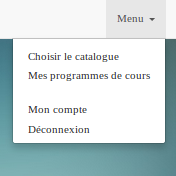
\includegraphics[scale=1]{student_landing_page_2}
\end{figure}
\section{Le choix du catalogue de cours}
Un catalogue de cours est un ensemble de programmes que la commission mets en ligne au début d'une année académique. Par défaut, le dernier en date est sélectionné pour votre profil. Cependant, vous pouvez décider pour une raison X ou Y de choisir votre programme dans un autre catalogue. Un étudiant a accès à deux types de catalogues: 


\begin{itemize}
\item un catalogue principal, qui est la version la plus actuelle mise à disposition par la commission de programme;
\item ceux dont la version est ancienne; ce sont des anciens catalogues \textit{principaux}.
\end{itemize}

Le formulaire qui permet de sélectionner le catalogue de cours est illustré sur la capture \ref{fig:choose_catalog_version}.

\begin{figure}
\centering
\caption{Choisir son catalogue de cours}
\label{fig:choose_catalog_version}
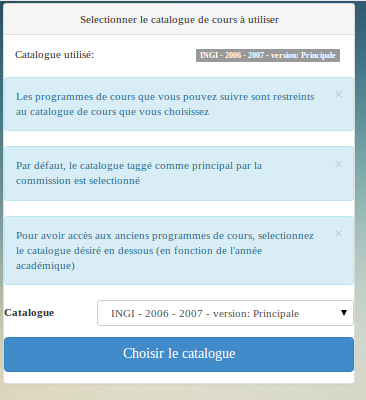
\includegraphics[width=\textwidth]{choose_catalog_version}
\end{figure}

Cette étape est optionnelle, en effet, à la création du compte, le catalogue principal est sélectionné par défaut. L'étudiant devrait quoiqu'il arrive utiliser ce catalogue.


\section{Le choix du programme de cours}
Pour créer son programme, l'étudiant doit tout d'abord sélectionner le programme de cours qu'il compte suivre (SINF1BA, SINF2M, FSA1BA, ...). Pour avoir plus d'information au niveaux des composantes (cours, modules, contraintes) d'un programme, l'étudiant doit se rendre dans le menu \textbf{Programmes disponibles} de la page illustrée sur la capture \ref{fig:student_landing_page_manual}. 

La page qui permet de naviguer à travers les différents programmes de cours proposés est illustré sur la capture \ref{fig:programs_availables}.

\begin{figure}[htb]
\centering
\caption{Programmes de cours proposés}
\label{fig:programs_availables}
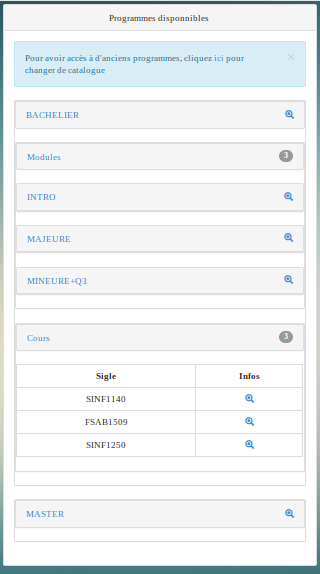
\includegraphics[height=0.9\textheight]{programs_available}
\end{figure}

Pour obtenir plus d'information sur un cours, module ou programme, il suffit de cliquer sur la petite loupe en \textcolor{blue}{bleu} à droite de chacun des onglets. 

\section{Configurer son programme de cours}

La page qui permet de gérer les différents programmes de l'étudiant est illustré sur la capture \ref{fig:student_program_index}:

\begin{itemize}
\item pour accéder à la configuration du programme, cliquer sur la petite loupe en \textcolor{blue}{bleu} en dessous du menu \textbf{Infos};
\item pour accéder au menu qui résume le statut de votre programme, les justifications que vous lui avez apporté et les commentaires ajoutés par la commission, cliquer sur la petite enveloppe en \textcolor{blue}{bleu} en dessous du menu \textbf{Justifications};
\item le menu \textbf{Validé?} indique si votre programme a été validé ou non par la commission de programme;
\end{itemize}

Pour créer un nouveau programme, cliquer sur le bouton \textbf{Nouveau Programme}.


\begin{figure}[htb]
\centering
\caption{Programmes de cours de l'étudiant}
\label{fig:student_program_index}
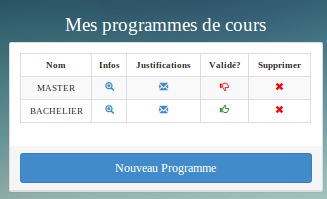
\includegraphics[width=\textwidth]{student_program_index}
\end{figure}

\subsection{Création du programme}

\begin{figure}[htb]
\centering
\caption{Création d'un programme de cours}
\label{fig:student_program_new}

\includegraphics[width=\textwidth]{student_program_new}
\end{figure}

L'étape de création (capture d'écran \ref{fig:student_program_new}) se résume à choisir le programme de cours que l'on veut suivre. Une fois le programme créé, vous arrivez sur la page illustrée sur la capture \ref{fig:student_program_mgmt}. Cliquez sur le bouton \textbf{Configurer le programme de cours} pour configurer les années et choisir les différents modules (options) qui constitueront votre programme.

\begin{figure}[htb]
\centering
\caption{Page de gestion d'un programme d'étudiant}
\label{fig:student_program_mgmt}
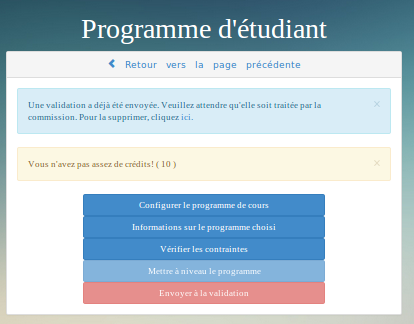
\includegraphics[width=\textwidth]{student_program_show}
\end{figure}

\subsection{Configuration du programme}
\subsubsection{Choisir les modules}
Un programme de cours est constitué de modules optionnels et obligatoires. Vous êtes obligé de choisir les modules obligatoires, et tout les cours qui les composent. Libre à vous de choisir un ou plusieurs modules optionnels. Certains modules comportent un sous-module qu'il est obligatoire de suivre si l'on choisir le module.

La page illustrée sur la capture \ref{fig:configure_modules} illustre cette fonctionnalité. À tout moment, vous pouvez modifier les modules que vous suivez. 

\begin{figure}[htb]
\centering
\caption{Choisir ses modules}
\label{fig:configure_modules}
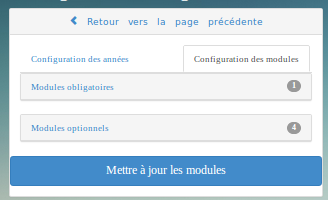
\includegraphics[width= \textwidth]{configure_modules}
\end{figure}

\subsubsection{Configurer les années}
Une fois le programme créé, il faut configurer les années qui composent ce programme.
\begin{figure}[htb]
\centering 
\caption{Configuration des années}
\label{fig:configure_years}
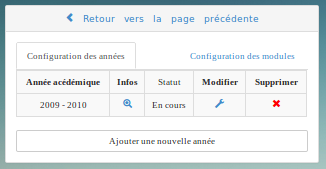
\includegraphics[width=\textwidth]{configure_years}
\end{figure}

Une année peut avoir trois statuts différents:
\begin{description}
\item[En cours] ; elle correspond à l'année dans laquelle vous vous trouvez actuellement (ou une année qui n'a pas encore été traitée par la commission);
\item[Ratée] ; elle correspond à une année qui n'a pas été réussie (les cours qui n'ont pas été crédités on été supprimés);
\item[Réussie] ; elle correspond à une année qui a été réussie.
\end{description}

Les années \textbf{réussies} et \textbf{ratées} ne sont plus modifiable ou supprimables!

La configuration d'une année est relativement simple, elle se déroule par semestre. Il suffit de choisir, l'année académique à laquelle l'année correspond et pour chaque semestre, les cours que vous désirez suivre parmi les cous obligatoires et optionnels disponibles (pour plus de détails, se référer à la capture \ref{fig:configure_years}).

\begin{figure}[htb]
\centering
\caption{Configuration d'une année}
\label{fig:configure_year}
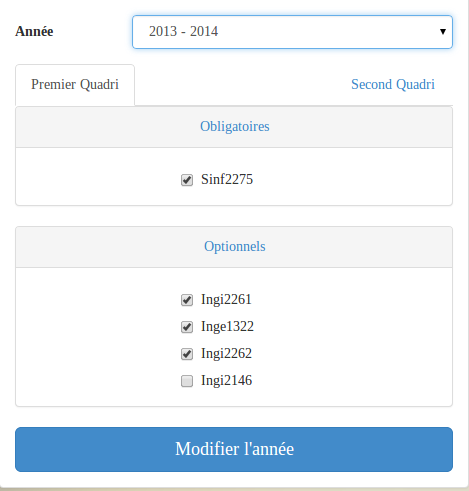
\includegraphics[width=\textwidth]{year_configuration}
\end{figure}



\subsubsection{Nouveau programme de cours disponible}
Au début d'une année académique, il est fort possible que la commission de programme mette en ligne une nouvelle version du catalogue de cours que vous utilisez. Il vous sera proposé de migrer le programme de cours que vous suivez vers la nouvelle version qui est disponible. 

Remarques:
\begin{itemize}
\item il se peut que le nom de certains cours change, ou que certaines contraintes changent aussi, ou même disparaissent. Le formulaire de justification, expliqué dans la sous-section qui suit, sert aussi à cet effet; il vous suffit juste d'expliquer que vous avez déjà suivi le cours en question, la commission s'occupera de vérifier que c'est bien le cas, et validera votre programme;
\item lorsque vous migrer votre programme de cours, le lien qui existe entre votre programme et les modules que vous avez décidé de suivre sera supprimer; il faudra donc aller les re-sélectionner dans le menu \ref{fig:configure_modules}. 
\end{itemize} 
\subsection{Vérification des contraintes - Justifications}

Pour vérifier les contraintes de votre programme, sélectionner le menu \textbf{Vérifier les contraintes} de la page illustrée sur la capture \ref{fig:student_program_mgmt}. 

La page de vérifications des contraintes est divisée en deux parties. 

En haut, la page illustrée sur la capture \ref{fig:student_program_status}. Elle affiche un résumé du statut de votre programme de cours, à savoir le nombre total de crédits qui le compose, si vous avez atteint le nombre de crédits minimaux ou si vous avez dépassé le nombre de crédits maximaux. 

En bas, la page illustrée sur la capture \ref{fig:student_program_justifications}. Toutes les contraintes que votre programme ne respecte pas sont affichées sur cette page, et les raisons pour lesquelles elles nes ont pas respectées. Vous êtes invité à résoudre ces exceptions en ajoutant les cours ou modules qui manquent. Pour toute les contraintes que vous ne pouvez pas résoudre, veuillez remplir la case justification prévue à cet effet, puis cliquer sur le bouton \textbf{Compléter la justification}.

À chaque fois que vous modifier votre programme, le formulaire de justification est remis à zéro. 

\begin{figure}[htb]
\centering
\caption{Statut du programme}
\label{fig:student_program_status}
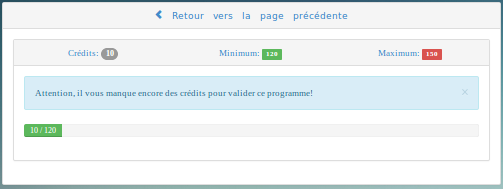
\includegraphics[width=\textwidth]{student_program_status}
\end{figure}

\begin{figure}[htb]
\centering
\caption{Statut des contraintes - Formulaire de justification}
\label{fig:student_program_justifications}
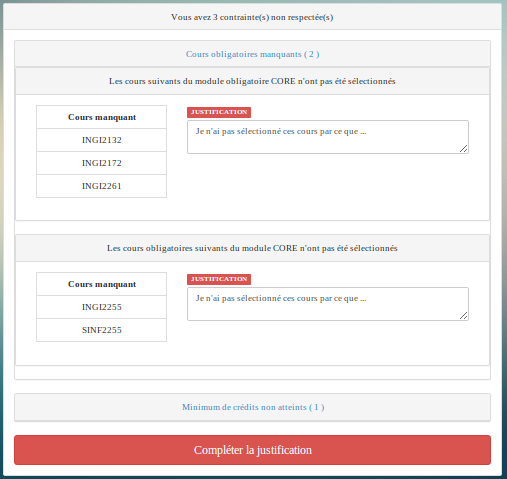
\includegraphics[width=\textwidth]{student_program_justifications}
\end{figure}

\subsection{Envoyer son programme à la validation}

Les conditions suivantes doivent être respectées afin de pouvoir envoyer une demande de validation;
\begin{description}
  \item[avoir assez de crédits] ; le programme de l'étudiant doit respecter le minimum de crédits requis par le programme qu'il suit (dans le cas ou le programme ne propose pas suffisamment de cours, il suffit d'avoir autant de crédits que le programme en propose)
  \item[avoir accédé au menu de gestion des contraintes] ; à chaque fois que l'étudiant modifie son programme, il lui est demandé d'avoir visité au moins une fois la page relative à la vérification des contraintes pour pouvoir soumettre son programme;
  \item[ne pas avoir de dépendances non respectées ou avoir rempli le formulaire de justification] ; si le programme de l'étudiant comporte des contraintes non respectées, il lui est demandé de remplir un formulaire de justification dans le quel il doit justifier chacune des exceptions (contraintes non respectées);
  \item[ne pas avoir une requête en cours] ; si une requête a déjà été envoyée pour le programme, il n'est pas possible d'en envoyer une nouvelle tant que la précédente n'a pas été refusée ou acceptée par la commission de programme. Pour ne pas bloquer l'étudiant et demander à la commission de programme de faire plusieurs fois le travail de vérification, l'étudiant peut à tout moment annuler sa demande de validation, modifier son programme puis la renvoyer. 
\end{description} 